\documentclass{article}

% packages
\usepackage{graphicx}
\usepackage{lastpage}
\usepackage{fancyhdr}
\usepackage[hidelinks]{hyperref}
\usepackage{color}
\usepackage{float}

% page margins
\addtolength{\topmargin}{-0.75in}
\addtolength{\oddsidemargin}{-1.0in}
\addtolength{\evensidemargin}{-1.0in}
\addtolength{\textwidth}{2.0in}
\addtolength{\textheight}{1.5in}

% header and footer
\pagestyle{fancy}
\fancyhf{}
\lhead{Fault-Tolerant Quadcopter}
\rhead{\textit{Vaughn, Mayank, Cooper}}
\cfoot{\thepage\ of \pageref{LastPage}}
\rfoot{\today}

% custom commands
\newcommand{\HREF}[2]{{\color{blue}\underline{\smash{\href{#1}{#2}}}}}

% metadata
\title{ECE 453 Project Proposal}
\author{Vaughn Kottler}
\author{Mayank Katwal}
\author{Cooper Green}

\begin{document}

\begin{center}

	{\huge\textbf{ECE 453 Project Proposal} (Fall 2018)}

	{\large University of Wisconsin-Madison}

	{\large\textit{Vaughn Kottler, Mayank Katwal, Cooper Green}}

\end{center}

\section{Introduction}

We are interested in building a \textit{quadcopter} plus
\textit{ground station} and \textit{web-based user interface}.
We have chosen to call this project the
\textbf{fault-tolerant quadcopter}. This name reveals one of our
design goals that will be covered in a future section.

This document serves as the formal proposal to be vetted by the
course instructor,
\HREF{https://directory.engr.wisc.edu/ece/Faculty/Krachey_Joe/}{Joe Krachey}.
We have
\HREF{https://fault-tolerant-quadcopter.readthedocs.io/en/latest/}
{additional documentation in work online} that we plan to keep in
sync with our project's scope and current progress. At the time
of writing it is not yet in a stable state.

This project is designed for three major bodies of work that were
mentioned above but are better captured by \textbf{Figure \ref{fig:high-level}}:

\begin{figure}[H]
	\centering
	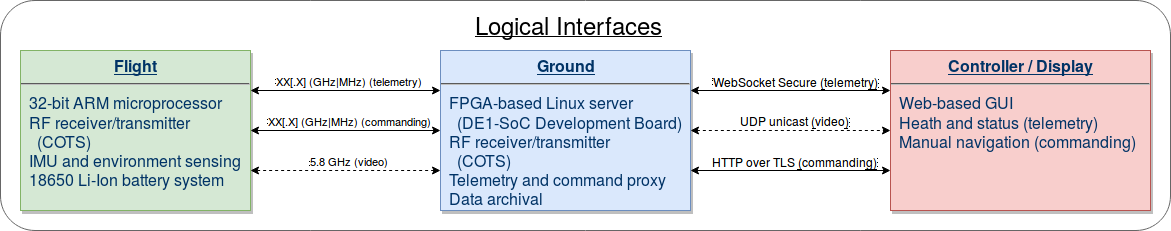
\includegraphics[width=\linewidth]{../src/im/top_level}
	\caption{High-level overview of the major components and
		their interfaces.}
	\label{fig:high-level}
\end{figure}

\noindent This high-level architecture is inspired by existing aerospace
avionics and software systems that we have done research on
and have some first-hand experience with. Our current, collective
experience with such systems (and the technical challenges we
anticipate being associated with them) is minimal, though. For
this reason \textbf{we seek feedback on our lower-level goals and
approach}, provided that this high-level idea suffices as
a project worth pursuing.

\section{Technical Features}

A vehicle that is \textit{single-fault tolerant} is capable of continuing
nominal operation after experiencing any arbitrary failure in a well-defined
\textit{fault space}. We aim to implement single-fault tolerance by:

\begin{enumerate}
	\item Limiting the initial fault space to a ``loss of ground station
		heartbeat'' event
	\item Executing a ``landing maneuver'' upon fault detection
	\item Iteratively hardening our design to a broader fault space,
		time permitting
\end{enumerate}

\noindent We recognize some intermediate milestones that will need to be reached
before an \textit{automatic flight-termination system} described above can be
expected to function:

\begin{itemize}
	\item Establish wireless communication between the vehicle and
		ground station
	\item Establish percentage-based throttle control over each motor
	\item Establish manual-commanding capability to the vehicle from a
		web-based user interface
	\item View live telemetry from a web-based user interface
	\item Sense angular velocity via gyroscope and force experienced via
		inertial measurement unit
	\item Develop a control algorithm to fly in a stable hover or
		holding pattern
	\item Extend control algorithm to control for velocity in three axes
		to achieve controlled motion
	\item Sense relative altitude
	\item Extend control algorithm to control for a specific \textit{delta-y}
		(perpendicular to ground plane) 
\end{itemize}

\noindent Our limited understanding of control theory and lack of experience in
general with avionics systems may limit what we can achieve in the end, but we
recognize this and have focused on primarily \textit{system-level} goals and
requirements versus specific technical requirements (battery life, thrust and
payload capability, etc.).

\subsection{Quadcopter}

For the flight vehicle, we intend to pursue an implmentation depicted in
\textbf{Figure \ref{fig:quadcopter}}:

\begin{figure}[H]
	\centering
	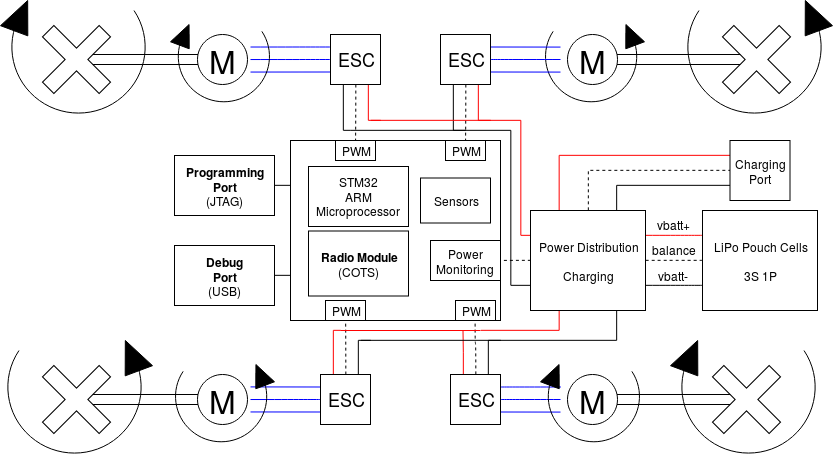
\includegraphics[width=\linewidth]{../src/im/quadcopter}
	\caption{Block diagram view of the quadcopter.}
	\label{fig:quadcopter}
\end{figure}

\noindent{\Large Responsible Engineer: \textbf{Vaughn}}

\pagebreak

\subsection{Ground Station}

For the ground station, we intend to pursue an implmentation depicted in
\textbf{Figure \ref{fig:ground_station}}:

\begin{figure}[H]
	\centering
	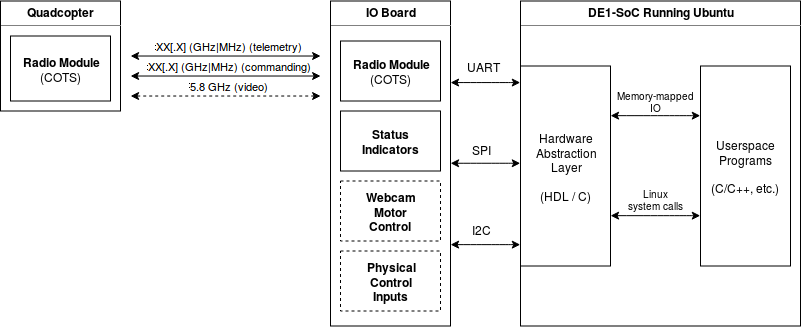
\includegraphics[width=\linewidth]{../src/im/ground_station}
	\caption{Block diagram view of the ground station.}
	\label{fig:ground_station}
\end{figure}

\noindent{\Large Responsible Engineer: \textbf{Cooper}}

\pagebreak

\subsection{Display and Controller}

For the display and control interface, we intend to pursue an
implmentation depicted in \textbf{Figure \ref{fig:display_controller}}:

\begin{figure}[H]
	\centering
	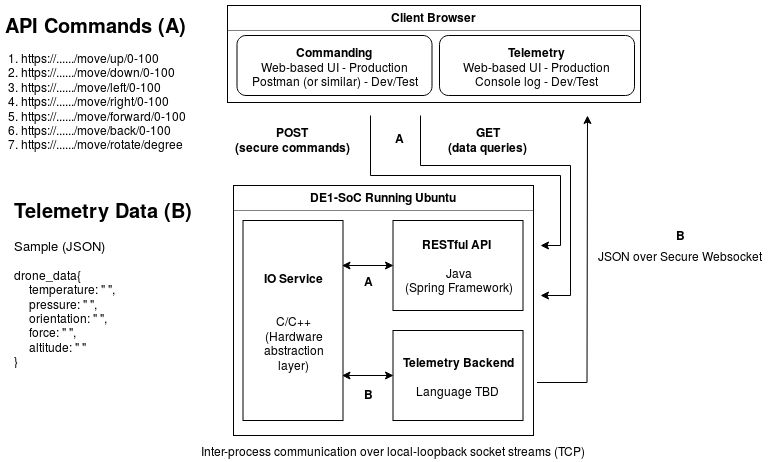
\includegraphics[width=\linewidth]{../src/im/display_controller}
	\caption{Block diagram view of the display and control user
		interface.}
	\label{fig:display_controller}
\end{figure}

\noindent{\Large Responsible Engineer: \textbf{Mayank}}

\section{Roles and Responsibilities}

\begin{quote}
	\textit{``A problem well stated is a problem half
	solved.'' - Charles Kettering}
\end{quote}

\noindent Distribution of work and responsibilities has been discussed and the
following summaries represent a consensus reached on initial roles and task
delegation.

\subsection{Vaughn Kottler}

\begin{description}
	\item [Flight Hardware] Final design and assembly of the quadcopter.
		Validation of component selection to ensure flight is feasible.
	\item [Flight Software] The firmware image flashed to the flight
		computer. Includes necessary control algorithms and runtime
		configurability.
	\item [Project Oversight] Track project progress and maintain
		documentation.
\end{description}

\subsection{Mayank Katwal}

\begin{description}
	\item [Telemetry Display] A web-based dashboard that summarizes the health
		and status of the quadcopter during flight.
	\item [Vehicle Control Interface] A web-based user interface that allows
		manual control of the quadcopter during flight.
	\item [Data and Command APIs] User programs that expose flight data
		and command capability to client browsers via HTTP over TLS requests.
\end{description}

\subsection{Cooper Green}

\begin{description}
	\item [Ground Station] Hardware asbstraction layer source code and
		mezzanine board implementation. A coherent and well-defined interface
		to the hardware from user programs.
	\item [Radio Frequency Communication] Choice of frequency bands and
		protocols used to send and receive data with radio modules.
	\item [Telemetry Storage] A data archival system for post-flight analysis.
\end{description}

\section{Project Management}

\begin{quote}
	\textit{``If I had an hour to solve a problem I'd spend 55 minutes
	thinking about the problem and 5 minutes thinking about
	solutions.'' - Albert Einstein}
\end{quote}

\noindent The value of detailed (but \textit{precise}!) planning for a project
of this scope and timeline cannot be overstated. Prototyping and experimenting
is inevitable but must be guided to avoid allocating disproportionate effort
towards minor goals that put higher-level goals at risk.
\textbf{Figure \ref{fig:workflow_1}} introduces our approach and
\textbf{Figure \ref{fig:workflow_2}} establishes a proposed process for
handling integration and final stages in project realization.

\begin{figure}[H]
	\centering
	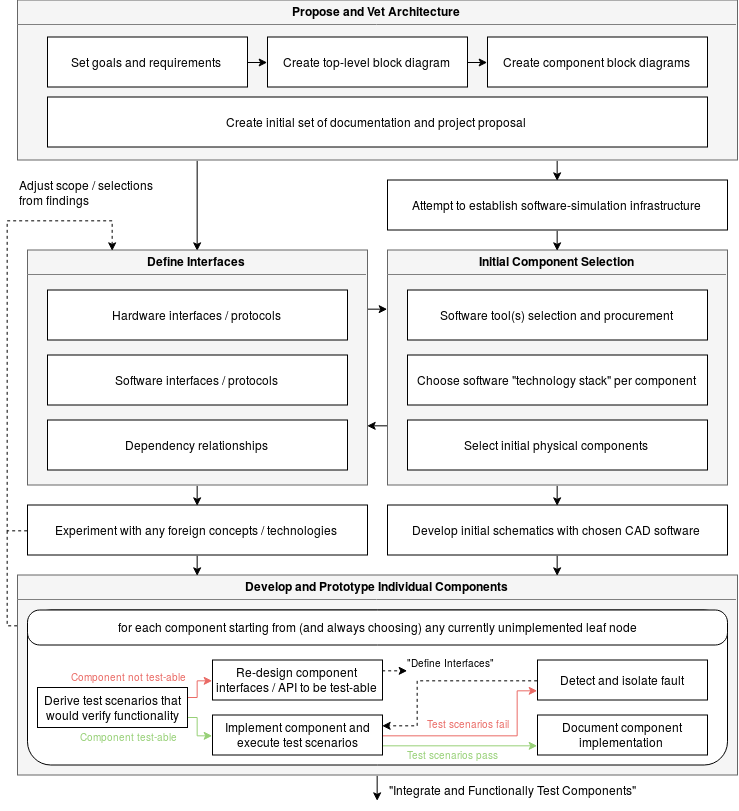
\includegraphics[width=\linewidth]{../src/im/workflow_1}
	\caption{A flexible workflow diagram that attempts to capture our ideal
		process for initial prototype and development work.}
	\label{fig:workflow_1}
\end{figure}

\begin{figure}[H]
	\centering
	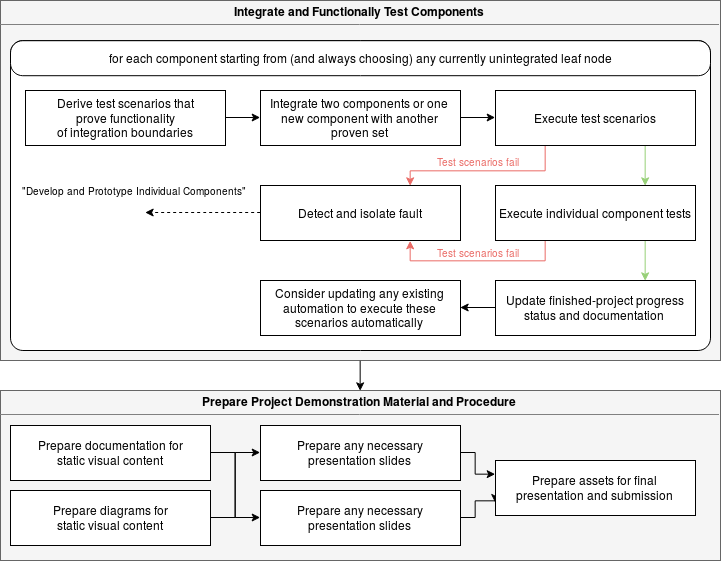
\includegraphics[width=\linewidth]{../src/im/workflow_2}
	\caption{The remaining stages of the workflow diagram that captures our
		intended process for bringing the project to completion.}
	\label{fig:workflow_2}
\end{figure}

\end{document}
